%!TEX root = ../physical-olympics-2.tex
\chapter{静磁学} 


\section{电流与磁场}

\subsection{磁场地位与电流分布}

人们对磁的认识一共经历了几个阶段:
\begin{enumerate}
\item 起: 远古-\emph{奥斯特}({\it H. C.\O rsted}). 磁现象被认为与\emph{磁体}(magnet)相关. 它被设想为由\emph{磁荷}(magnetic charge)造成.
\item 承: 奥斯特-\emph{麦克斯韦}({\it J. C. Maxwell}). 奥斯特发现了电流的磁效应, \emph{法拉第}({\it M. Faraday})建立了``场''的观念, 可以定量描述电流产生的磁场, 法拉第与\emph{亨利}({\it J.Henry})等人发现了电磁感应, \emph{安培}({\it A.-M. Amp\`ere})的\emph{分子电流假说}解释了物质磁性的本质也是电流产生磁场.
\item 转: 麦克斯韦-\emph{狄拉克}({\it P. Dirac}). 麦克斯韦和\emph{洛伦兹}({\it H. A. Lorentz})给出了电磁场的普遍理论, 即\emph{电动力学}(electrodynamics)\footnote{这个词语却是安培发明的.}, 洛伦兹和\emph{爱因斯坦}({\it A. Einstein})等人将电动力学纳入相对论框架. \emph{赫兹}({\it H. R. Hertz})的实验有效地支持了电磁场论. 洛伦兹等人的经典电子论是微观粒子与电磁场之间相互作用的第一个完备理论, 微观粒子被陆续发现, 电子的\emph{自旋}(spin)与\emph{磁矩}(magnetic moment)被发现与研究.
\item 合: 狄拉克-现今. 狄拉克主张把电子量子化为场, 提出了\emph{量子电动力学}(quantum electrodynamics), 预言了反物质的存在, \emph{安德森}({\it C. D. Anderson})实验室发现正电子. 狄拉克提出了量子化的\emph{磁单极子}(magnetic monopole)模型, 但至今未找到磁单极子.
\end{enumerate}

现在, 我们对\emph{磁场}(magnetic field)概念的理解就可以用下图来概括:

\begin{wrapfigure}[13]{o}[-10pt]{6cm}
\centering
\vspace{-0.7cm}
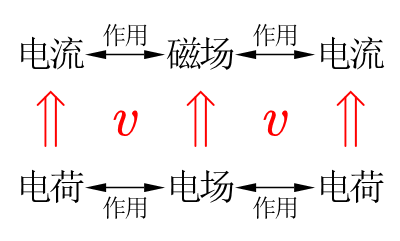
\includegraphics[width=6cm]{image/7-4-3.png}
\caption{磁场与电荷的关系}

\end{wrapfigure}

如何证明磁场是电场的相对论效应? 设想原参考系中只有电场, 那么无论原参考系中的速度$v_x,\,v_y,\,v_z$如何, 受力都不取决于速度大小, 它是:
\[F_x=qE_x\]
\[ F_y=qE_y \]
\[  F_z=qE_z\]

根据相对论的力变换公式:
\[F_x'=F_x-\frac{u}{c^2}\cdot\frac{v_yF_y+v_zF_z}{1-\frac{uv_x}{c^2}}\quad ,\quad F_y'=\frac{F_y}{\gamma (1-\frac{uv_x}{c^2})}\quad ,\quad F_z'=\frac{F_z}{\gamma (1-\frac{uv_x}{c^2})}\]

代入原式, 并假设原参考系速度和变换速度相对$c$都是小量, 故新参考系速度可以使用经典的速度叠加:
\[v_x=v_x'+u\quad ,\quad v_y=v_y' \quad ,\quad v_z=v_z'\]

近似到与$v_x',\,v_y',\,v_z'$一阶相关的领头项:

\[F_x'=qE_x-qv_y'\cdot \frac{uE_y}{c^2}-qv_z'\cdot \frac{uE_z}{c^2}\]
\[F_y'=qE_y+qv_x'\cdot \frac{uE_y}{c^2}\]
\[F_z'=qE_z+qv_x'\cdot \frac{uE_z}{c^2}\]

我们如果假设以下\emph{洛伦兹力}(Lorentz force)公式的成立性:
\[\bs{F}=q(\bs{E}+\bs{v}\times \bs{B})\]

它是磁场力分量$\bs{F}_m=q\bs{v}\times \bs{B}$与电场力分量$\bs{F}_e=q\bs{E}$的和. 则受力公式简化为:
\[F_x'=qE_x'+qv_y'B_z'-qv_z'B_y'\]
\[F_y'=qE_y'+qv_z'B_x'-qv_x'B_z'\]
\[F_z'=qE_z'+qv_x'B_y'-qv_y'B_x'\]

对比即知道:
\[B_x'=0\quad ,\quad B_y'=\frac{uE_z}{c^2} \quad ,\quad B_z'=-\frac{uE_x}{c^2}\]

这实际上是:
\[\bs{B}=-\frac{\bs{u}\times \bs{E}}{c^2}\]

如果原参考系是静止点电荷产生的电场, 现在换参考系以后, 点电荷做速度为$-\bs{u}$的匀速直线运动而产生以上磁场, 那么就能推理出, 如果点电荷以速度$\bs{v}$做匀速直线运动, 那么它产生的磁场必然为:
\[\bs{B}=\frac{1}{4\pi \varepsilon_0 c^2}\frac{q\bs{v}\times \bs{e}_r}{r^2}\]

我们从中总结出:
\begin{itemize}
	\item 只有运动的电荷才会受到磁场力.
	\item 只有运动的电荷才产生磁场.
	\item 但是运动与静止具有相对性, 所以电场和磁场的区别就像静止与运动的区别那样是相对的, 合称\emph{电磁场}(electromagneto field).
\end{itemize}

我们还注意到来自理论推导过程中产生的重要公式:

\[\bs{B}=\frac{1}{4\pi \varepsilon_0 c^2}\frac{q\bs{v}\times \bs{e}_r}{r^2}\]
\[\bs{F}=q\bs{v}\times \bs{B}\]

由于推导的近似性这两个式子似乎没有太多说服力. 但是历史上这两个式子是作为实验规律先被总结, 再有麦克斯韦的普遍电磁理论, 最后才是洛伦兹和爱因斯坦对其背后的相对论基础的研究.


\subsection{毕奥-萨伐尔定律}

强调一下本章研究的范围是重要的. 我们暂时只研究\emph{静磁场}(static magnetic field), 其场源为电流, 且其分布不随时间, 从而改变的磁场也不随时间改变. 或者更简单的说, 我们要研究的体系就是上一章建立的稳恒电流体系, 它由不变的电荷产生不变的电场, 不变的电场驱动不变的电流, 现在增加了不变的电流产生不变的磁场这一要素. 上一章的讨论告诉我们这就是要求电流分布是无散的:
\[\nabla \cdot \bs{j}=0\]

如何把微观电荷的运动同宏观的电流$\bs{j},\,I$建立联系? 引言中我们指出来过, 微观运动电荷产生的磁场正比于量:
\[\bs{C}=q\bs{v}\]

这个量被称作\emph{电流元}(current element). 事实上作为微观电荷$q$通常是基本电荷$e$的量级, 从而上述量是一个微元, 即使取物质中一个很小的体积$\ud V$, 其内部包含的所有电荷个数$\ud N$依然未达到宏观量级时, 总的电流元依然是个小量, 记做$\ud\bs{C}$. 我们知道电流密度的定义为:
\[\bs{j}=\rho\bs{v}=nq\bs{v}\]

那么体积产生的总的电流元:
\[\ud \bs{C}=\ud N q\bs{v}=nq\bs{v}\ud V=\bs{j}\ud V=\rho\ud V\cdot\bs{v}\]

称为\emph{体电流元}(volume current element). 同理, 我们可以写出\emph{面电流元}(surface current element)和\emph{线电流元}(curve current element):
\[\ud \bs{C}=\bs{i}\ud A=\sigma\bs{v}\ud A\quad ,\quad \ud \bs{C}=I\ud \bs{l}=\lambda \bs{v}\ud l\]

注意上面线电流元的写法, 由于我们不认为$I$是矢量, 故把电流元的矢量性由线元$\ud \bs{l}$来承载. 这么做的好处之后就能体会到. 我们发现电流元与电荷元形成了对应关系:
\begin{figure}[H]
\centering
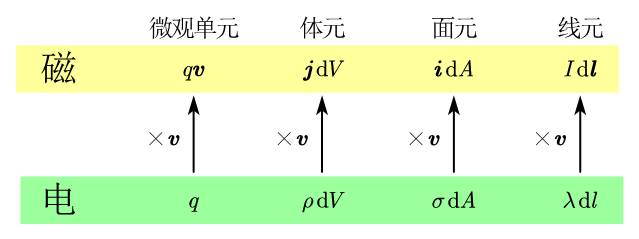
\includegraphics[width=0.6\textwidth]{image/7-4-4.png}
\caption{电荷元与电流元对应}
\end{figure}

\begin{wrapfigure}[10]{o}[-10pt]{6cm}
\centering
\vspace{-1cm}
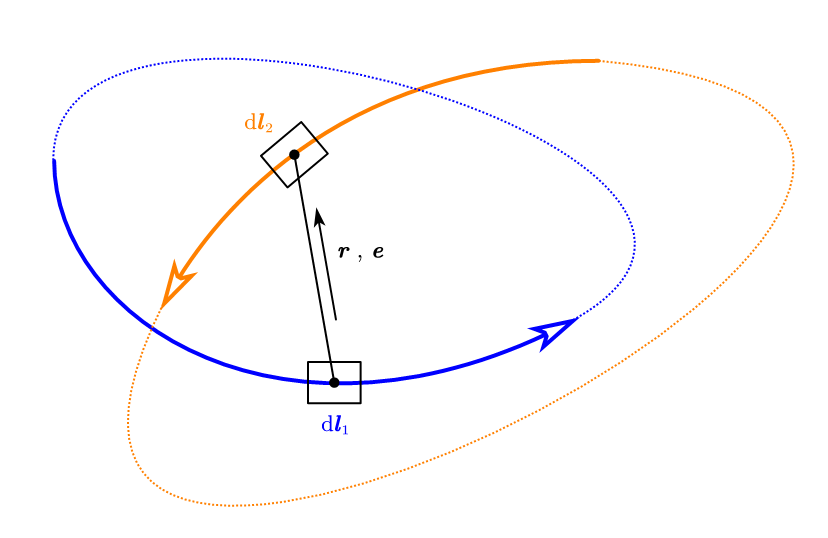
\includegraphics[width=6cm]{image/7-4-5.png}
\caption{电流体系间的相互作用力}
\end{wrapfigure}
$\phantom{0}\!\!\!$\emph{毕奥-萨伐尔定律}(Biot-Savart law)是一个实验定律, 它用于描述真空中两个孤立的电流元之间的相互作用力:
\[\ud \bs{F}_{12}=\frac{\mu_0}{4\pi}\frac{I_2\ud \bs{l}_2\times (I_1\ud \bs{l}_1\times \bs{e}_{12})}{r^2}\]

其中系数$k_m=\dfrac{\mu_0}{4\pi}\approx 1\times 10^{-7}{\rm H/m}$\footnote{注意, 2019年5月20日之后, 新的国际单位制标准下其值为$1.000\;000\;000\;82(20)\times 10^{-7}{\rm H/m}$, 不再有严格的$\mu_0:=4\pi\times 10^{-7}{\rm H/m}$.}为磁力常数, 而$\mu_0$称作\emph{真空磁导率}(magnetic permeability of vacuum). 事实上:
\[k_e/k_m=c^2\quad \text{或者}\quad c=\frac{1}{\sqrt{\varepsilon_0\mu_0}}\]

$c$是真空中的光速. 这也揭示了电磁理论统一性背后的相对论本质. 我们这里还用到了电感的国际单位亨利, 而磁场的国际单位\emph{特斯拉}(Tesla)与它的关系为:
\[1{\rm H}=1{\rm T\cdot m^2/A}\]

另一个常用的单位来自CGS单位制, 即\emph{高斯}(Gauss), 以纪念这位伟大的数学家在物理学上同样瞩目的贡献. 高斯在历史上被广泛使用, 直至今天也如此, 例如地表地磁场大概就在$0.25-0.60{\rm G}$, 它与特斯拉的换算关系为:
\[1{\rm T}=10000{\rm G}\]

根据场论的精神, 我们将上式拆解为电流产生场的定律和电流在场中受力的公式:
\[\ud \bs{F}_{12}=I_2\ud \bs{l}_2\times \ud \bs{B}_{12}\quad ,\quad \ud \bs{B}_{12}=\frac{\mu_0}{4\pi}\frac{I_1\ud \bs{l}_1\times \bs{e}_{12}}{r^2}\]

\begin{wrapfigure}[15]{o}[-10pt]{6cm}
\centering
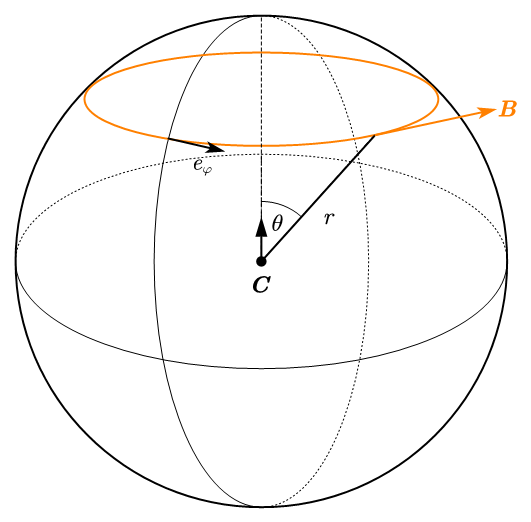
\includegraphics[width=6cm]{image/7-4-6.png}
\caption{电流元产生的磁场}
\end{wrapfigure}
如前所述, 毕奥-萨伐尔定律可以在相对论背景下由库仑定律推出, 故它继承了库仑定律的平方反比和叠加原理的特性. 但是它突出的特点是具有\emph{横向力}(transverse force)的特点: 力的方向与受力物体电流元垂直, 也与另一个只依赖于场源的磁场矢量垂直, 但这个矢量又与场源电流元的方向垂直. 两次叉乘这让力的计算变得比较复杂. 让我们以场源电流元$\bs{C}$为中心, 其方向建立极坐标系, 那么磁场的大小与方向就可以从公式得到:
\[\bs{B}=\kb\frac{C\sin\theta}{r^2}\bs{e}_\varphi \]

磁场符合叠加原理, 例如一个载流线圈, 源点坐标$\bs{r}'$, 场点坐标$\bs{r}$, 记$\bs{R}=\bs{r}-\bs{r}'$, $\ud \bs{l}=\ud \bs{r}'$, 则其产生的磁场公式为:
\[\bs{B}=\oint \kb\frac{I\ud \bs{l}\times \bs{e}_{\bs{R}}}{R^2}\]



\begin{figure}[H]
\centering
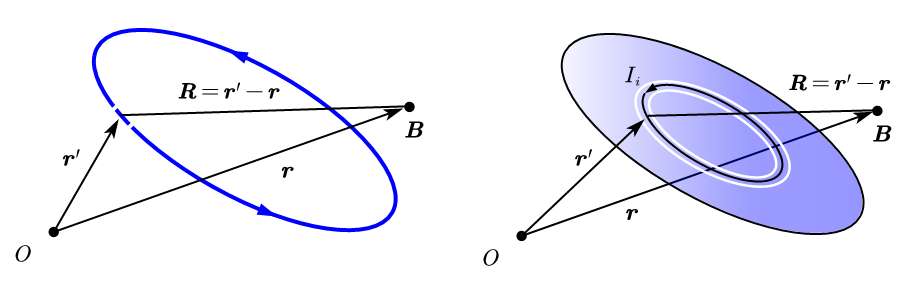
\includegraphics[width=0.8\textwidth]{image/7-4-7.png}
\caption{连续体系产生磁场}
\end{figure}

载流线圈具有非常重要的地位, 任何体电流分布, 只要是有界区域内的稳恒电流, 电流线就必然构成闭合的回路. 那么就一定可以分解为电流圈. 如果用求和的极限表示积分但是暴力地省去极限符号, 此时磁场计算方法为:
\[\bs{B}=\int\limits_{V'} \kb\frac{\bs{j}\times \bs{e}_{\bs{R}}}{R^2}\ud V=\sum_i \oint \kb\frac{I_i\ud \bs{l}_i\times \bs{e}_{\bs{R}}}{R^2}\]

而一个线圈或一个体电流分布在外磁场中的受力为:
\[\bs{F}=\oint I\ud\bs{l}\times \bs{B}\quad \Rightarrow\quad \bs{F}=\sum_i I_i\ud\bs{l}_i\times \bs{B}\]

在稳恒电流情况下, 讨论一个电流元产生的磁场是没有意义的, 因为空间的磁场必然是整个体系产生的磁场的叠加, 从而单个电流元的磁场并不具有可观测的意义, 除非电流可以独立的被操控以改变. 而讨论一个电流体系各个部分受到的作用力时, 尤其是一个电流线圈受到的作用力时, 区分内力和外力就变得尤其重要. 我们发现, 两个电流元之间的相互作用力之和:
\[\ud \bs{F}_{12}+\ud \bs{F}_{21}=\frac{\mu_0}{4\pi}\frac{I_2\ud \bs{l}_2\times (I_1\ud \bs{l}_1\times \bs{e}_{12})}{r^2}+\frac{\mu_0}{4\pi}\frac{I_1\ud \bs{l}_1\times (I_2\ud \bs{l}_2\times \bs{e}_{21})}{r^2}\]

根据三重矢积公式$\bs{A}\times(\bs{B}\times\bs{C})=(\bs{A}\cdot\bs{C})\bs{B}+(\bs{A}\cdot\bs{B})\bs{C}$, $\bs{e}_{12}=-\bs{e}_{21}$. 得到:
\[\ud \bs{F}_{12}+\ud \bs{F}_{21}=-\kb \frac{(I_1\ud \bs{l}_1\times I_2\ud \bs{l}_2)\times \bs{e}_{12}}{r^2}\]

一般来说不总为零, 可见朴素的牛顿第三定律在静磁场情况下失效了. 我们不得不把$\ud\bs{F}_{12},\,\ud \bs{F}_{21}$不再视作相互作用力, 而是需要通过场作为媒介. 事实上两个运动电荷之间的磁场力是在作为电场力的相对论修正, 从相对论的根本原理上, 相互作用传递速度的有限性导致力的传播被推迟, 原则上也不可能符合牛顿第三定律.

但是如果我们计算两个线圈之间的相互作用力之和:
\begin{align*}
\delta\bs{F}&=\oint\limits_1\oint\limits_2\ud \bs{F}_{12}+\oint\limits_2\oint\limits_1\ud \bs{F}_{21}\\
&=\frac{\mu_0I_1I_2}{4\pi}\left(\oint\limits_1\oint\limits_2\frac{(\bs{r}_2-\bs{r}_1)\cdot\ud(\bs{r}_2-\bs{r}_1)}{|\bs{r}_2-\bs{r}_1|^3}\ud\bs{r}_1+\oint\limits_2\oint\limits_1\frac{(\bs{r}_1-\bs{r}_2)\cdot\ud(\bs{r}_1-\bs{r}_2)}{|\bs{r}_1-\bs{r}_2|^3}\ud\bs{r}_2\right)
\end{align*}

但是:
\[\nabla_2 \frac{1}{|\bs{r}_2-\bs{r}_1|}=-\frac{\bs{r}_2-\bs{r}_1}{|\bs{r}_2-\bs{r}_1|^3}\quad\Rightarrow\quad \oint\limits_2\frac{(\bs{r}_2-\bs{r}_1)\cdot\ud(\bs{r}_2-\bs{r}_1)}{|\bs{r}_2-\bs{r}_1|^3}=0\]
\[\nabla_1 \frac{1}{|\bs{r}_1-\bs{r}_2|}=-\frac{\bs{r}_1-\bs{r}_2}{|\bs{r}_1-\bs{r}_2|^3}\quad\Rightarrow\quad \oint\limits_1\frac{(\bs{r}_1-\bs{r}_2)\cdot\ud(\bs{r}_1-\bs{r}_2)}{|\bs{r}_1-\bs{r}_2|^3}=0\]

从而得到:
\[\delta\bs{F}=0\]

当两个环重合时, 这也代表``自己给自己的力''是零. 即使是磁场给线圈的力, 也因为是线圈自己产生的磁场而无法对自己产生力, 这个结果其实也是空间平移对称性(而不是牛顿第三定律)的必然结果. 而空间旋转对称性则给出, 任意选取$O$点计算各个电流元受力对$O$的力矩, 总和必然为零. 或者说两个线圈之间的作用力与作用力矩之间必然符合牛顿第三定律. 其证明在此不再赘述. 这样我们就证明了此前给出的理论公式与牛顿第三定律之间是自洽的, 无散的电流体系下牛顿第三定律依然成立, 尽管表面上电流元的毕奥萨伐尔定律与牛顿第三定律有冲突.

更有甚者, 我们指出, 根据麦克斯韦方程的协变性, 即使是微观电荷做相对论性运动, 只要是稳恒电流体系, 那么毕奥萨伐尔定律可以作为一个推论而具有普适性. 而对于非稳恒体系, 后面我们将会证明, 磁场此时并不能简单地由电流确定而依赖于电场的变化率, 甚至它成为了自由存在的物质形式而摆脱了电荷造成的任何约束.

\section{两个定律与矢势}

\subsection{磁场的环路定律}

静磁场的\emph{环路定律}(circuital law), 又称\emph{安培定律}(Amp\`ere's law)指出, 对于一个可定向曲面$\bs{A}$和它的闭合右手边界$\partial\bs{A}$, 有:
\[\oint\limits_{\partial \bs{A}}\bs{B}\cdot \ud \bs{l}=\mu_0 \int\limits_{\bs{A}}\bs{j}\cdot \ud \bs{A}\]

我们用毕奥-萨伐尔定律来证明环路定律. 首先, 上式中的$A$和其边界上的场点位矢取为$\bs{r}$, 则$\ud \bs{l}=\ud\bs{r}$, 而场源电流分解为电流环$I_i$. 将电流环上坐标选为$\bs{r}'$. 那么以上积分可按照叠加原理分解为:
\[\Gamma=\sum_i \Gamma_i=\sum_i\oint\limits_{\partial \bs{A}}\bs{B}_i\cdot \ud \bs{l}\]

而每一项环量就可以用场点和源点的两次环积分表示, 将$\bs{e}_R$记做$\bs{e}$:
\begin{align*}
\Gamma_i 	&=\oint\limits_{\bs{r}}\bs{B}_i\cdot \ud \bs{r}\\
			&=\oint\limits_{\bs{r}}\left(\oint\limits_{\bs{r}'} \kb\frac{I_i\ud \bs{r}'\times \bs{e}_{\bs{R}}}{R^2}\right)\cdot \ud \bs{r}\\
			&=\frac{\mu_0I_i}{4\pi} \oint\limits_{\bs{r}}\oint\limits_{\bs{r}'}\frac{(\ud \bs{r}\times \ud \bs{r}')\cdot \bs{e}_{\bs{R}}}{R^2}
\end{align*}

\begin{figure}[H]
\centering
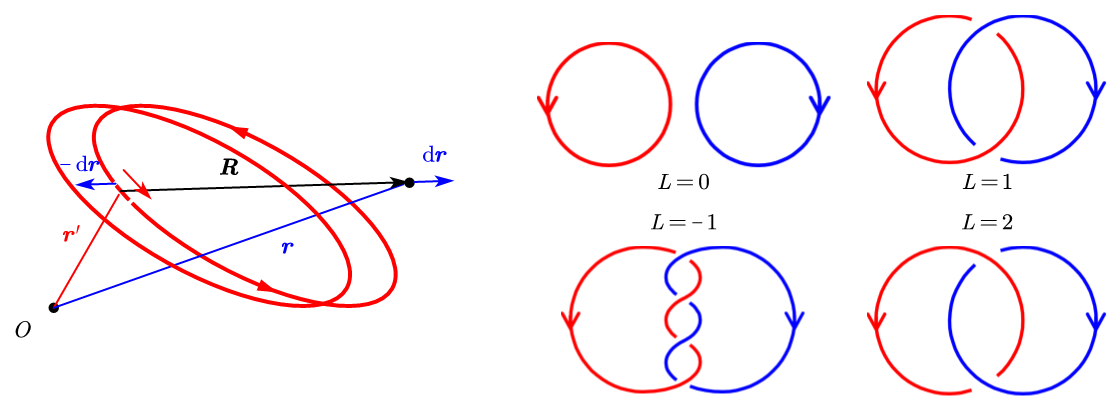
\includegraphics[width=0.9\textwidth]{image/7-4-8.png}
\caption{环绕数}\label{fig:7-4-8}
\end{figure}

如上图所示, 对上面的积分做如下诠释: 当从场点$\bs{r}$去看线圈时, 线圈对场点产生了一个立体角$\Omega$. 当观察点移动$\ud\bs{r}$时, 考察立体角的改变$\ud \Omega$. 可以等效地把线圈反向移动$-\ud\bs{r}$. 图中所示情况立体角将减小, 算法为:
\[-\ud\Omega=\int\frac{\ud \bs{A}\cdot (-\bs{e}_{\bs{R}})}{R^2}=\oint\limits_{\bs{r}'}\frac{(-\ud \bs{r}\times \ud \bs{r}') \cdot (-\bs{e}_{\bs{R}})}{R^2}\]

下面考虑以源电流圈(\ref{fig:7-4-8}中红圈)为边界的那个面, 场点形成的安培回路(\ref{fig:7-4-8}中蓝圈)与这个面的交点个数为$n_1+n_2$, 其中$n_1$代表蓝圈正向穿过面时方向与红圈形成右手规则的交点个数, $n_2$代表蓝圈正向穿过面时方向与红圈形成左手规则的交点个数. 于是再定义\emph{环绕数}(linking number):
\[\ell=n_1-n_2\]

这是一个拓扑学不变量, 它只取决于两个回路的整理性质, 与面的取法无关, 而且具有对称性(红对蓝与蓝对红的环绕数一致).

从而我们注意到, 如果环绕数恰好是一, 那么从面上出发, $\Omega$从一个接近$2\pi$的大小一直在减小直到变为零, 然后变成负的, 直到回到面上直到变成接近$-2\pi$, 虽然初末位置立体角不一定都等于$2\pi$, 但是一定有:
\[\oint\limits_{\bs{r}}\ud\Omega=-4\pi\]

相似的, 如果考虑一个环绕数为$L$的安培回路, 就有:
\[\oint\limits_{\bs{r}}\ud\Omega=-4\pi \ell\]

将此前的立体角微分代入, 得到:
\[\oint\limits_{\bs{r}}\oint\limits_{\bs{r}'}\frac{(\ud \bs{r}\times \ud \bs{r}')\cdot \bs{e}_{\bs{R}}}{R^2}=4\pi \ell\]

最后代入此前的磁场环量, 得到:
\[\Gamma_i=\mu_0\ell_iI_i\]

最后我们总结出:
\[\oint\limits_{\partial \bs{A}}\bs{B}\cdot \ud \bs{l}=\mu_0\sum_i \ell_iI_i\]

现在做极限化处理, 注意到求和式实际上就是统计了所有以右手规则为正向通过面的电流, 统一用电流密度表示就变成了自带正负的点乘的积分:
\[\oint\limits_{\partial \bs{A}}\bs{B}\cdot \ud \bs{l}=\mu_0 \int\limits_{\bs{A}}\bs{j}\cdot \ud \bs{A}\]

此即环路定律, 由数学上的开尔文-斯托克斯定理, 我们可以把上式写出局域的微分形式:
\[\nabla\times \bs{B}=\mu_0 \bs{j}\]


\subsection{矢势与磁场的高斯定律}

对电流元产生的磁场$\ud \bs{B}=\dfrac{\mu_0}{4\pi}\dfrac{\bs{j}\ud V\times \bs{e}_r}{ r^2}$引入以下矢量场是方便的:
\[\bs{A}=\frac{\mu_0}{4\pi}\frac{\bs{j}\ud V}{r}\]

这是因为如果计算球坐标下的旋度, 考虑到$\bs{A}$分解到$r,\,\theta$方向分别为:
\[A_r=\frac{\mu_0}{4\pi}\frac{j\ud V}{r}\cos\theta\quad ,\quad A_\theta=-\frac{\mu_0}{4\pi}\frac{j\ud V}{r}\sin\theta\]

那么考虑一个回路\footnote{为了避免与磁矢势符号重复, 暂时用$S$表示面元.}$S:\,(r,\,\theta)-(r+\ud r,\,\theta)-(r+\ud r,\,\theta+\ud \theta)-(r,\,\theta+\ud \theta)-(r,\,\theta)$, 利用旋度的定义式:
\[\bs{n}\cdot\nabla\times \bs{A}=\left.\lim_{S\to 0}\oint\limits_{\partial S}\bs{A}\cdot \ud \bs{l}\right/S\]

得到其旋度:
\[\nabla\times \bs{A}=\frac{1}{r}\left(\frac{\partial rA_\theta}{\partial r}-\frac{\partial A_r}{\partial \theta}\right)\bs{e}_\varphi\]

代入便得到以下关系式:
\[\bs{B}=\frac{\mu_0}{4\pi}\frac{j\ud V}{r^2}\sin\theta\bs{e}_\varphi=\nabla\times \bs{A}\]

$\bs{A}$这个矢量称作\emph{磁矢势}(magnetic vector potential). 由于叠加原理, 一个电流分布体系的磁矢势和磁场应当为:
\[\bs{A}=\int\limits_V \frac{\mu_0}{4\pi}\frac{\bs{j}\ud V}{r}\quad ,\quad \bs{B}=\int\limits_V \frac{\mu_0}{4\pi}\frac{\bs{j}\ud V\times \bs{e}_r}{r^2}\]

同样地将满足:
\[\bs{B}=\nabla\times \bs{A}\]

以上旋度关系写成积分形式意味着一种计算磁通量的特殊方法:
\[\Phi=\oint\limits_{\partial S} \bs{A}\cdot \ud \bs{l}=\int\limits_S\bs{B}\cdot \ud \bs{S}\]


对于无边界的闭合曲面, 上式直接证明了磁场\emph{高斯定律}(Gauss's law):
\[\partial\partial V=\emptyset\quad\Rightarrow\quad \oint\limits_{\partial V}\bs{B}\cdot \ud \bs{S}=\oint\limits_{\partial\partial V} \bs{A}\cdot \ud \bs{l}=0\]
\[\Rightarrow\quad  \nabla\cdot \bs{B}=0\]

我们如果计算此前电流元产生的磁矢势的散度:
\[\nabla\cdot\bs{A}=\nabla\cdot\left(\frac{\mu_0}{4\pi}\frac{j\ud V}{r}\bs{e}_z\right)=\frac{\mu_0}{4\pi}j\ud V\frac{\partial}{\partial z}\left(\frac{1}{r}\right)=\frac{\mu_0}{4\pi}\frac{j\ud V\cos\theta}{r^2}=\frac{\mu_0}{4\pi}\frac{j\ud V\cdot \bs{e}_r}{r^2}\]

又发现对电流元得到非零的结果. 但是如果考虑线圈:
\[\nabla\cdot\bs{A}=\oint \frac{\mu_0}{4\pi}\frac{I\ud \bs{l}\cdot \bs{e}_{\bs{R}}}{R^2}=\frac{\mu_0 I}{4\pi}\oint \frac{\bs{e}_{\bs{R}}}{R^2}\cdot \ud \bs{r}'=\frac{\mu_0 I}{4\pi}\oint \nabla_{\bs{r}'}\left(\frac{1}{R}\right)\cdot \ud \bs{R}=\frac{\mu_0 I}{4\pi}\oint \ud\left(\frac{1}{R}\right)=0\]

从而对于任意稳恒电流体系, 通过此前积分定义的磁矢势也是无散的. 最后将磁矢势与磁场关系和磁场与电流关系联立, 注意到:
\[\nabla\times(\nabla\times \bs{A})=\nabla(\nabla\cdot\bs{A})-\nabla^2\bs{A}\]

即三重矢积公式. 我们把梯度算符$\nabla$直接看作了一个矢量. 上式右侧第一项由于磁矢势无散故为零, 从而得到:
\[\nabla^2\bs{A}=-\mu_0\bs{A}\]

电场中的式子$\nabla^2\varphi=-\rho/\varepsilon_0$与它相呼应.


可以设想存在可以像点电荷产生电场那样的方式产生磁场的物质, 称作\emph{磁单极子}(magnetic monopole), 从而可以产生不为零的净\emph{磁荷}(magnetic charge), 事实证明这样的物质至今都未曾找到, 从而相伴的磁场形式也仅仅存在与理论中. 但是, 总磁荷为零的体系: \emph{磁偶极子}(magnetic dipole), 不仅仅是纯粹的理论模型, 后面可以发现线圈产生的磁场与磁偶极子是相似的.

我们记得电势可以被视作电荷在电场中运动的势能有关的物理量, 即$E_p=q\varphi$. 那么电荷在磁场中运动时, 磁矢势代表什么物理概念呢? 如果空间中只有纯的磁场, 那么显然磁场力不做功:
\[P=\frac{\ud W}{\ud t}=\bs{F}_m\cdot \bs{v}=(q\bs{v}\times\bs{B})\cdot\bs{v}=0\]

所以电荷一定是动能不变的. 但是即使如此, 我们也不认为磁场力是一个保守力, 这是因为保守力的定义应该是: 能够用势能的梯度来表示的作用力. 我们写出一个项:
\[\bs{\pi}=q\bs{A}\]

这个项不再具有能量的量纲而是动量的量纲. 我们知道电场除磁场的量纲为速度, 而两者与对应的矢势标势都差一个长度量纲, 故$q\bs{A}$量纲等于用$q\varphi$的能量量纲除速度, 即动量量纲. 这个动量称为\emph{势动量}(potential momentum). 而带电粒子的旧动量$\bs{p}=m\bs{v}$就称作\emph{机械动量}(kinetic momentum), 它是运动造成的, 而势动量是位置$\bs{r}$造成的$\bs{\pi}(\bs{r})$, 是与磁场相互作用引起的动量. 两者之和:
\[\bs{P}=\bs{p}+\bs{\pi}\]

称作\emph{正则动量}(canonical momentum). 不像在电场中的电荷运动机械能(动能+势能)守恒, 这个和也是一般不守恒的:
\begin{align*}
\dot{\bs{P}}	&=\dot{\bs{p}}+\dot{\bs{\pi}}\\
				&=\bs{F}+q\dot{\bs{A}}\\
				&=q\bs{v}\times(\nabla\times \bs{A})+q\bs{v}\cdot\nabla\bs{A}\\
				&=-\nabla(-q\bs{v}\cdot\bs{A})
\end{align*}

最后一步把$\nabla$视作矢量使用了三重矢积公式. 注意到瞬时的$\bs{v}$不被视作变量而视作常数而从偏导数符号内外移动不引起改变. 我们发现瞬时的正则动量导数似乎恰好等于某个势能的负梯度:
\[V=-q\bs{v}\cdot\bs{A}\]

这被称作\emph{广义势}(generalized potential). 它含有速度, 从而每一个时刻有着完全不同的形式. 但不管怎样, 粒子在磁场中的运动的确是写成了一个动量导数等于势的梯度的形式(拉格朗日方程形式). 即使这样, 我们依然不认为磁场力是一个保守力.

\begin{wrapfigure}[15]{o}[-10pt]{6cm}
\centering
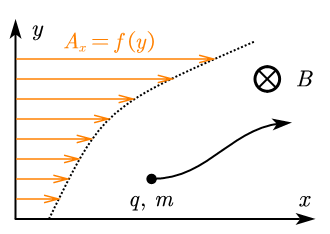
\includegraphics[width=6cm]{image/7-4-9.png}
\caption{正则动量守恒}
\end{wrapfigure}
我们来看一个具体的例子. 假设空间中的电流分布产生了一个随$y$方向变化的$x$方向的磁矢势分布:
\[\bs{A}=(f(y),\,0,\,0)=f(y)\bs{e}_x\]

那么可以验证这个式子的确符合:
\[\nabla\cdot\bs{A}=\frac{\partial f(y)}{\partial x}=0\]

而产生它的电流和对应的磁场就是:
\[\bs{j}=-\nabla^2\bs{A}/\mu_0=-\frac{1}{\mu_0}\left(\frac{\partial^2}{\partial x^2}+\frac{\partial^2}{\partial y^2}+\frac{\partial^2}{\partial z^2}\right)f(y)\bs{e}_x=-\frac{f''(y)}{\mu_0}\bs{e}_x\]
\[\bs{B}=\nabla\times \bs{A}=-\frac{\partial f(y)}{\partial y}\bs{e}_z=-f'(y)\bs{e}_z\]

这表示一个垂直$x-y$平面的磁场. 那么粒子在某一瞬时的广义势:
\[V=-q\bs{v}\cdot\bs{A}=-qv_xf(y)\]

其瞬时梯度就是:
\[-\nabla V=-qv_xf'(y)\bs{e}_y\]

而粒子的正则动量是:
\[\bs{P}=(mv_x+qf(y))\bs{e}_x+mv_y\bs{e}_x\]

根据此前的论述:
\[\dot{\bs{P}}=-\nabla V\]

从而我们发现, 在$x$方向粒子的\emph{广义动量守恒}(concervation of generalized momentum):
\[mv_x+qf(y)={\rm Const.}\]

而在$y$方向有一动力学方程:
\[ma_y=-qv_xf'(y)\]

读者可以用牛顿力学同样的论证以上两个式子的成立性.


\section{电流体系}

研究更进一步的磁场与电流相互作用的模型前, 熟悉一些常见的电流体系的结论是大有裨益的, 这些包括:

\subsection{磁偶极子}

同样类似于对静电学中一个分布在原点附近的电流体系在远场产生的电势进行展开的思想, 我们此时运用到静磁学情形: 计算一个分布在原点附近的电流体系在远场产生的磁矢势:
\[\bs{A}=\int\limits_{V'}\kb \frac{\bs{j}\ud V'}{|\bs{r}-\bs{r}'|}\]
利用分解为线圈可以简化以上计算:
\[\bs{A}=\sum_i\oint\kb \frac{I_i\ud\bs{l}_i}{|\bs{r}-\bs{r}_i|}\]

依然利用静电学中的展开公式:
\begin{align*}
\frac{1}{|\bs{r}-\bs{r}_i|} 	&=[(\bs{r}-\bs{r}_i)^2]^{-\frac{1}{2}}=(\bs{r}^2-2\bs{r}_i\cdot\bs{r}+\bs{r}_i^2)^{-\frac{1}{2}} \\
								&\approx (\bs{r}^2-2\bs{r}_i\cdot\bs{r})^{-\frac{1}{2}}=\frac{1}{r}\left(1-2\frac{\bs{r}_i\cdot\bs{r}}{r^2}\right)^{-\frac{1}{2}} \\
								&\approx \frac{1}{r}\left(1+\frac{\bs{r}_i\cdot\bs{r}}{r^2}\right)\\
								&=\frac{1}{r}+\frac{\bs{e}_r}{r^2}\cdot \bs{r}_i 
\end{align*}

代入上式, 注意到$\ud\bs{l}_i=\ud \bs{r}_i$得到磁矢势展开的前两项:
\[\bs{A}\approx\frac{\mu_0}{4\pi r}\sum_i I_i\oint\ud \bs{r}_i+\frac{\mu_0}{4\pi r^2}\sum_i I_i\oint(\bs{e}_r\cdot \bs{r}_i)\ud \bs{r}_i\]

第一项由于对回路积分必然为零. 第二个积分中需要注意$\bs{e}_r$照理应当是可以提取到积分号外面的常矢量, 但是这样积分内部的$\bs{r}_i\ud \bs{r}_i$构成了一个不直观的张量. 我们采用一个更加简单的做法: \emph{常矢量点乘法}(method of dot product by a constant vector). 任意取一个常矢量$\bs{v}$来点乘积分结果:
\[\bs{v}\cdot\oint(\bs{e}_r\cdot \bs{r}_i)\ud \bs{r}_i=\oint(\bs{e}_r\cdot \bs{r}_i)(\bs{v}\cdot\ud \bs{r}_i)=\bs{e}_r\cdot \oint(\bs{v}\cdot\ud \bs{r}_i)\bs{r}_i\]

这样倒是可以实现$\bs{e}_r$移到积分外, 但代价是另一个类似的$\bs{v}$又到了积分内. 其实无济于事. 但是注意到中间的积分其实完全可以使用开尔文-斯托克斯定理:
\[\oint(\bs{e}_r\cdot \bs{r}_i)(\bs{v}\cdot\ud \bs{r}_i)=\oint\left[(\bs{e}_r\cdot \bs{r}_i)\bs{v}\right]\cdot\ud \bs{r}_i=\int\limits_{\bs{S}_i}\nabla\times\left[(\bs{e}_r\cdot \bs{r}_i)\bs{v}\right]\cdot\ud \bs{S}_i\]

根据叉乘的定义:
\[\nabla\times\left[(\bs{e}_r\cdot \bs{r}_i)\bs{v}\right]=\begin{vmatrix}
\frac{\partial}{\partial x} &\frac{\partial}{\partial y}&\frac{\partial}{\partial z}\\
(\bs{e}_r\cdot \bs{r}_i)v_x &(\bs{e}_r\cdot \bs{r}_i)v_y&(\bs{e}_r\cdot \bs{r}_i)v_z\\
\bs{e}_x&\bs{e}_y&\bs{e}_z
\end{vmatrix}\]

其中$\bs{e}_r=(e_{rx},\,e_{rx},\,e_{rx})$和$(v_x,\,v_y,\,v_z)$都是常的. 故求偏导只发生在点乘式$\bs{e}_r\cdot \bs{r}_i$中的一项上给出不为零的系数. 即:
\[\nabla\times\left[(\bs{e}_r\cdot \bs{r}_i)\bs{v}\right]=\begin{vmatrix}
e_{rx}&e_{rx}&e_{rx}\\
v_x &v_y&v_z\\
\bs{e}_x&\bs{e}_y&\bs{e}_z
\end{vmatrix}=\bs{e}_r\times\bs{v}\]

最终得到:
\[\bs{v}\cdot\oint(\bs{e}_r\cdot \bs{r}_i)\ud \bs{r}_i=\int\limits_{\bs{S}_i}\left(\bs{e}_r\times\bs{v}\right)\cdot\ud \bs{S}_i=\bs{v}\cdot\left[\left(\int\limits_{\bs{S}_i}\ud\bs{S}_i\right)\times\bs{e}_r\right]=\bs{v}\cdot\left(\bs{S}_i\times\bs{e}_r\right)\]

由于工具$\bs{v}$的任意性, 现在就可以看出以下关系:
\[\oint(\bs{e}_r\cdot \bs{r}_i)\ud \bs{r}_i=\bs{S}_i\times\bs{e}_r\]

再代入此前的磁矢势, 得到最终结果:
\[\bs{A}\approx\frac{\mu_0}{4\pi r^2}\left(\sum_i I_i\bs{S}_i\right)\times\bs{e}_r\]

\begin{wrapfigure}[22]{o}[-10pt]{6cm}
\centering
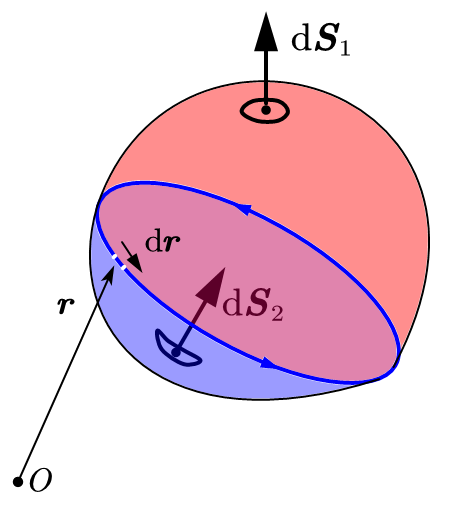
\includegraphics[width=6cm]{image/7-4-10.png}
\caption{线圈与面矢量}\label{fig:7-4-10}
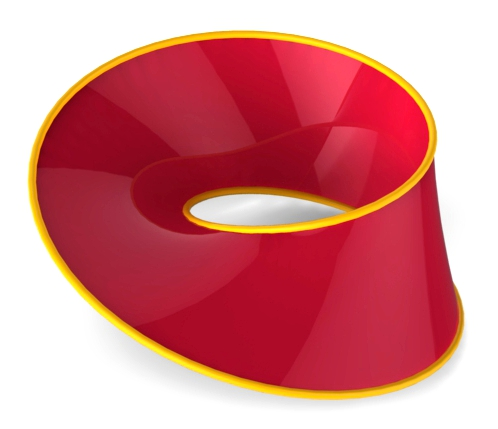
\includegraphics[width=6cm]{image/7-4-11.jpg}
\caption{莫比乌斯带}\label{fig:7-4-11}
\end{wrapfigure}
在讨论最终结果前我们对上式出现的一种现象需要做进一步的解释. 如图\ref{fig:7-4-10}所示, 一个线圈对应的面矢量$\bs{S}$的标准定义实际上对应着以下线圈上的路径积分:
\[\bs{S}=\frac{1}{2}\oint\bs{r}\times \ud \bs{r}\]

这样定义也绝非完美, 我们自然觉得, 一个线圈对应的面矢量的确定应该是与坐标原点选取无关的, 但上式在表面上有关. 如果原点位移了$\bs{R}$, 两个积分的差为:
\begin{align*}
\bs{S}'	&=\frac{1}{2}\oint\left(\bs{r}-\bs{R}\right)\times \ud (\bs{r}-\bs{R})\\
			&=\frac{1}{2}\oint\left(\bs{r}-\bs{R}\right)\times \ud \bs{r}\\
			&=\bs{S}-\frac{1}{2}\bs{R}\times\oint\ud \bs{r}\\
			&=\bs{S}
\end{align*}
	
故以上定义的确不依赖于原点的选取. 但是我们要问, 为什么上式就表示以线圈为边界的面矢量呢? 而这样定义又有何好处? 事实上, 如过按照通常的方式来定义一个边界所确定的面的面矢量, 那么就面临着一个奇怪的问题: 不同的面可能共用了同一个边界, 甚至会出现莫比乌斯带那样, 一个简单的闭合曲线却以一个反常的不可定向的面的边界的形式出现了, 我们甚至可以在一个圆环作为边界的情况下构造出莫比乌斯带型的不可定向曲面来, 将莫比乌斯带的边界扯成一个圆环即可. 为了避免这种情况, 我们最好是用曲线积分来定义面矢量, 这样对于复杂曲线(比如自己打结的曲线, 比如螺旋线)也不必受难以确定以其为边界的曲面之苦. 事实上, 如果对于\ref{fig:7-4-10}那样的曲线较为简单的情况, 选取以其为边界的可定向曲面, 依然把右手定则确定的微元面矢量积分定义为整个面的面矢量, 那么对于\ref{fig:7-4-10}中两个不同的面:
\[\bs{S}_1=\int\limits_{\bs{S}_1}\ud \bs{S}_1\quad ,\quad \bs{S}_2=\int\limits_{\bs{S}_1}\ud \bs{S}_2\]


我们自然也要问, 以上两个积分是否会相等? 事实上如果把两个积分相减, 就得到了在一个体的闭合表面上的面元积分:
\[\bs{S}_1-\bs{S}_2=\oint\limits_{\partial V}\ud\bs{S}\]

要想得到上式的值, 我们又再一次使用常矢量点乘法:
\[\bs{v}\cdot(\bs{S}_1-\bs{S}_2)=\oint\limits_{\partial V}\bs{v}\cdot\ud\bs{S}\]

很显然, 这表示一个常矢量场在闭合面上的通量, 如匀强电场通过一个闭合面的电通量代数和, 从而一定是零. 由$\bs{v}$的任意性, 总有:
\[\bs{S}_1-\bs{S}_2=0\quad ,\quad \bs{S}_1=\bs{S}_2\]

从而这个定义也是不依赖于曲面的选取的, 而为了把之前标准定义的曲线积分和对面元的积分联系起来, 我们再使用常矢量点乘法:
\[\bs{v}\cdot\frac{1}{2}\oint\limits_{\partial\bs{S}}\bs{r}\times \ud \bs{r}=\frac{1}{2}\oint\limits_{\partial \bs{S}}(\bs{v}\times\bs{r}) \cdot \ud \bs{r}=\frac{1}{2}\int\limits_{\bs{S}}\nabla\times(\bs{v}\times\bs{r}) \cdot \ud \bs{S}\]

利用$\bs{v}$为常矢量时可以在$\nabla$前后移动的特性, 得到:
\[\nabla\times(\bs{v}\times\bs{r})=(\nabla\cdot \bs{r})\bs{v}-(\bs{v}\cdot\nabla)\bs{r}=3\bs{v}-\bs{v}=2\bs{v}\]

代入上式:
\[\bs{v}\cdot\frac{1}{2}\oint\limits_{\partial\bs{S}}\bs{r}\times \ud \bs{r}=\frac{1}{2}\int\limits_{\bs{S}}2\bs{v} \cdot \ud \bs{S}=\bs{v} \cdot\int\limits_{\bs{S}}\ud \bs{S}\]

从而就证明的确这个曲线积分就是面矢量:

\[\frac{1}{2}\oint\limits_{\partial\bs{S}}\bs{r}\times \ud \bs{r}=\int\limits_{\bs{S}}\ud \bs{S}=\bs{S}\]

关于用曲线积分得到总的面矢量$\bs{S}$还有一种几何理解方式, 再仔细观察图\ref{fig:7-4-10}就会发现, 项:
\[\frac{1}{2}\bs{r}\times \ud \bs{r}\]

实际上就是原点$O$出发向曲线上的一段$ \ud \bs{r}$连线形成的三角形面元, 它恰好是从$O$出发向曲线上的所有点引射线形成的锥面上的一个面元, 故积分就得到整个锥面的总面矢量且与曲线环绕方向恰好符合右手规则, 它也是一种特殊的以曲线为边界的面的总面矢量.

终于我们回到此前电流体系形成的磁矢势问题, 现在我们就定义一个载流$I_i$的线圈形成的\emph{磁矩}(magnetic moment)为:
\[\bs{m}_i=I_i\bs{S}_i\]

而这个电流体系形成的总磁矩就是:
\[\bs{m}=\sum_i \bs{m}_i=\sum_iI_i\bs{S}_i\]

那么在远场的磁矢势的领头项就是由磁矩产生的平方反比项:
\[\bs{A}=\frac{\mu_0}{4\pi}\frac{\bs{m}\times \bs{e}_r}{r^2}\]

这个式子其实非常类似电流元$\bs{C}$产生的磁场公式:
\[\bs{B}=\frac{\mu_0}{4\pi}\frac{\bs{C}\times \bs{e}_r}{r^2}\]

但是要计算磁矩产生的磁场, 应对以上形式的磁矢势来求旋度, 计算可得:
\[B_r=\frac{\mu_0}{4\pi}\frac{2m\cos\theta }{r^3}\quad ,\quad B_\theta=\frac{\mu_0}{4\pi}\frac{m\sin\theta }{r^3}\]

也许令人惊讶的是, 其关于$r,\,\theta$变化的形式居然与电偶极子产生的电场的公式一致\footnote{其实这个形式是拉普拉斯算符, 或者说, 背后的对称性导致的必然结果}.

磁矩产生的磁场具有非常重要的地位, 第一是因为任何情况下这都会是一个电流体系激发的磁场的领头项, 因为磁单极子不存在, 类似点电荷产生平方反比的电场那样的磁荷项, 由于磁高斯定律, 永远是不可能的. 磁矩的计算方式上面已经给出, 但是我们依然要指出, 将求和再还原为对提电流的积分, 可以得到磁矩的体积分算法:
\[\bs{m}=\frac{1}{2}\int\limits_V \bs{r}\times \bs{j}\ud V\]

而最简单的磁矩模型就是一个平面圆环, 其电流为$I$, 半径为$R$. 那么磁矩就是:
\[m=I\pi R^2\]

而考虑$I\to \infty, S\to 0$的模型, 就构成了\emph{点磁偶极子}(point dipole)的情况. 此时体系产生的磁场将严格符合我们得出的三个计算式:
\[\bs{A}=\frac{\mu_0}{4\pi}\frac{\bs{m}\times \bs{e}_r}{r^2}\quad ,\quad B_r=\frac{\mu_0}{4\pi}\frac{2m\cos\theta }{r^3}\quad ,\quad B_\theta=\frac{\mu_0}{4\pi}\frac{m\sin\theta }{r^3}\]

第二, 任何稳恒电流体系可以向线圈分解, 而任何线圈又可以向磁偶极子来分解. 我们把载有电流$I$的线圈所在的可定向曲面分解为无穷多无穷小的网格, 并让每一个网格都载有同样的方向的电流$I$, 那么网格形成的总电流分布实际上就是原线圈的电流分布, 因为有公共边的两个网格在公共边上的电流一定恰好反向而产生的电流互相抵消, 最后只剩下最外面的一圈边界上电流被保留下来. 从而不管是产生的场还是在外场中的受力均可以用于等效原来的线圈.

磁偶极子的磁势能, 受力与力矩:
\[V=-\bs{m}\cdot \bs{B}\quad ,\quad \bs{F}=\bs{m}\cdot \nabla\bs{B}\quad ,\quad \bs{M}=\bs{m}\times \bs{B}\]



\subsection{磁化强度}

\begin{itemize}
\item \emph{磁化强度}(magnetization):
\[\bs{M}=n\bs{m}\]

\item 磁化强度造成的体电流与面电流分布:
\[\bs{j}_M=\nabla\times \bs{M}\quad ,\quad \bs{i}_M=\bs{M}\times \bs{n}\]


\end{itemize}

\subsection{若干对称体系的磁场}

\begin{itemize}
\item 无限长载流直线:
\[\bs{A}=-\frac{\mu_0 I}{2\pi}\ln r\quad ,\quad \bs{B}=\frac{\mu_0 I}{2\pi r}\bs{e}_\varphi\]

\begin{figure}[H]
\centering
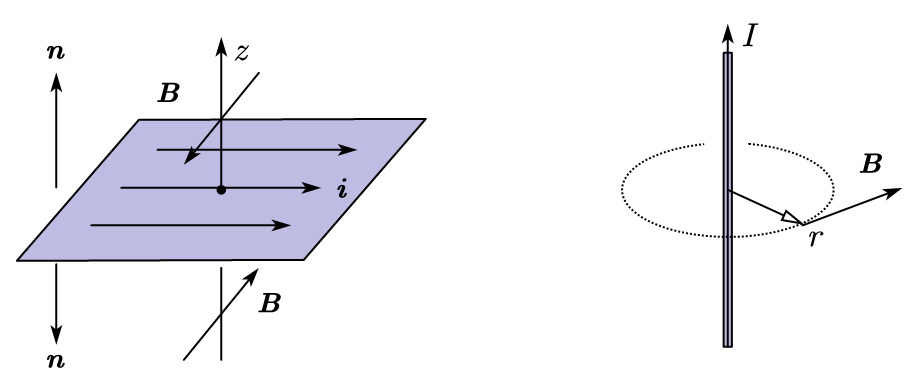
\includegraphics[width=0.7\textwidth]{image/7-4-1.png}
\caption{无限大平面与无限长直线}\label{fig7-4-1}
\end{figure}

\item 无限大载流平面:
\[\bs{B}=\frac{1}{2}\mu_0\bs{i}\times \bs{n}\]

\item 圆环: 半径为$R$的标准载流线圈轴线上磁场:
\[\bs{B}=\frac{\mu_0IR}{2(R^2+z^2)^{\frac{3}{2}}}\bs{e}_z\]

该处的径向场强可以由磁高斯定理确定:
\[\frac{1}{2}\frac{\ud B_r}{\ud r}+\frac{\ud B_z}{\ud z}=0\quad \Rightarrow \quad B_r\approx -\frac{3\mu_0IRzr}{(R^2+z^2)^{\frac{5}{2}}}\]

\item 无限长密绕螺线管: 无论其横截面形状, 总是有:
\[B=\mu_0 i=\mu_0 nI=\frac{\mu_0 NI}{l}\]
\end{itemize}


\section{磁介质与磁能}

\subsection{微观角度理解磁化}

\begin{itemize}
\item 分子的固有磁矩: 电子自旋磁矩+电子轨道磁矩.
\item 如果分子具有固有磁矩, 那么按照热力学规律发生取向磁化: 磁矩倾向于取与外磁场相同的方向, 宏观上产生\emph{顺磁性}(paramagnetism). 类似于电介质的极化, 微观上顺磁磁化规律可以写作:
\[\bar{\bs{\mu}}=\alpha \bs{B}\]
\item 电子的磁矩与角动量的比称为\emph{旋磁比}(gyromagnetic ratio), 轨道旋磁比与自旋旋磁比分别为:
\[\gamma_L=-\frac{e}{2m_e}\quad ,\quad \gamma_S=-\frac{e}{m_e}\]

角动量量子化理论告诉我们, $z$方向上电子轨道与自旋角动量只能为:
\[L_z=\pm n\hbar \quad ,\quad  S_z=\pm \frac{\hbar}{2}\]

故$z$方向上的磁矩的单位就是著名的\emph{玻尔磁子}(Bohr magneton):
\[\mu_B=\frac{e\hbar}{2m_e}=0.00579{\rm meV/T}\]

事实上由于自旋-轨道耦合, 分子磁矩可以是玻尔磁子的分数倍.

\item 原子核也有磁矩, 显然由于质子质量比质子质量大三个量级, 故根据旋磁比算法, 其磁矩也小三个量级. 虽然对分子磁矩和宏观磁化几乎没有贡献, 但是利用在磁场下形成的各个能级间跃迁吸收发射电磁辐射的原理可以造成\emph{核磁共振}(nuclear magnetic resonance)现象.

\item 如果分子的固有磁矩为零, 那么在外磁场下会产生一个与外磁场反向的磁矩, 宏观上造成\emph{抗磁性}(diamagnetism). 从微观来看似乎与电介质极化的方向相反, 但是从宏观效果上却与电介质削弱电场的效果相同, 这是电与磁固有的区别导致的.

\item 抗磁性的微观起源为电子轨道运动的\emph{拉莫尔进动}(Larmor precession). 由轨道运动产生的力矩, 角动量, 磁矩三者关系可得:
\[\bs{M}=\bs{\mu}\times \bs{B}\quad ,\quad  \bs{\mu}=\gamma \bs{L}\quad ,\quad  \frac{\ud}{\ud t}\bs{L}=\bs{M}\]
\[\Rightarrow \quad  \frac{\ud}{\ud t}\bs{L}=-\gamma \bs{B}\times \bs{L}=\frac{e\bs{B}}{2m}\times \bs{L}\]

故在运动学上, 电子将以以下角速度发生进动:
\[\bs{\Omega}=\frac{e}{2m}\bs{B}\]

电子原来的轨道运动半径如果按照玻尔半径$a_0$估计, 而角动量量级为$\hbar$, 那么现在附加的角速度与原来的角速度的比为:
\[\Omega/\omega\sim\frac{ea_0^2}{2\hbar}B\]

故产生的磁矩与原来的玻尔磁子的比值的量级也与之相当, 得到磁矩的量级为:
\[\bar{\bs{\mu}}\sim-\frac{e^2a_0^2	}{4m}\bs{B}\]

系数便是抗磁性磁化的分子磁化率的量级, 它一般比顺磁性磁化要小一到两个量级.

\item 有一些金属, 或者特殊的金属化合物具有独特的\emph{铁磁性}(ferromagnetism), 微观上它们由介观的包含大量原子的\emph{磁畴}(magnetic domains)构成. 每一个磁畴由于单元之间的关联已经超过了热力学的涨落而成为了决定性的因素, 使得所有电子的自旋几乎都严格指向同一个方向, 磁化达到饱和. 而材料的磁化过程其实是不同的磁畴在外磁场下的转向. 它的磁化率将远远大于简单的顺磁和抗磁磁化. 而且体现出非线性和历史相关性.


\end{itemize}

\subsection{宏观角度理解磁化}

\begin{itemize}
\item 出于$\bs{B}$和$\bs{M}$的旋度分别为总电流密度和磁化电流密度, 引入\emph{磁场强度}(magnetic field strength)以区别于以往一贯描述磁场的$\bs{B}$, 一般可区别称作\emph{磁通密度}(magnetic flux density):
\[\bs{H}=\frac{\bs{B}}{\mu_0}-\bs{M}\]

这样这个矢量的旋度就只取决于外电流:
\[\nabla\times \bs{H}=\bs{j}_f\]

\item 在顺磁或铁磁的柱状介质外绕制密绕螺线管, 那么没有介质时其磁通密度为:
\[B_0=\mu_0 i\]

那么, 由于此时加入介质时磁化电流不影响$\bs{H}$的计算, 故磁场强度为:
\[H=\frac{B_0}{\mu_0}=i\]

但是磁化电流的存在将产生一个与原磁场同向的附加磁场, 使得介质内部的磁场变大, 那么定义此时磁场与原磁场的比值为\emph{相对磁导率}(relative magnetic permeability):
\[B/B_0=\mu_r\]

那么把绝对磁导率定义为$\mu=\mu_r\mu_0$, 就有以下关系式:
\[B=\mu H=\mu i\]

\[M=(\mu_r-1)H=\chi_m H\]

其中$\chi_m$就是宏观的\emph{磁化率}(magnetic susceptibility). 对于抗磁性物质, 其值是小于零的.


\end{itemize}

\subsection{磁场能量}

磁场体系的能量的计算方法可以证明可以有用电流与矢势和用能量密度两种计算方法:
\[I=\frac{1}{2}\int \bs{j}\cdot\bs{A}\ud V=\int \frac{1}{2\mu_0}	\bs{B}^2\ud V\]

同样地, 两个体系同时存在时, 体系将产生自能与相互作用能. 如两个电感元件如果之间存在互感, 那么其总能量应当为:
\[E=\frac{1}{2}L_1I_1^2+\frac{1}{2}L_2I_2^2+ MI_1I_2\]

如果存在介质, 其能量密度需要加上磁化带来的能量, 能量密度变为:
\[w=\frac{1}{2\mu}	\bs{B}^2=\frac{1}{2}\mu \bs{H}^2 =\frac{1}{2}	\bs{B}\cdot \bs{H}\]

%\section{超导简介}
